% Opener for November 4, 2026: who sat where? (five-chair seating puzzle)
% Build: pdflatex who-sat-where.tex, then copy to ../2026-11-04-opener.pdf
% Every puzzle here is checked for exactly one answer by check.py.
\documentclass[11pt]{article}
\usepackage[letterpaper,margin=0.5in]{geometry}
\usepackage[T1]{fontenc}
\usepackage[default]{sourcesanspro}
\usepackage{tikz}
\pagestyle{empty}
\setlength{\parindent}{0pt}
\definecolor{cgreen}{HTML}{1F7A3A}\definecolor{cbrown}{HTML}{7B4A2B}
\definecolor{cred}{HTML}{D83A3A}\definecolor{cyellow}{HTML}{F2C318}
\definecolor{corange}{HTML}{F28A1E}
% \chairs{list of colour/name/number}
\newcommand{\chair}[3]{% x, colour, label
  \fill[#2!35!white,draw=#2!80!black,line width=1pt,rounded corners=3pt] (#1,0) rectangle ++(3.1,1.5);
  \node[font=\bfseries] at (#1+1.55,0.75) {#3};
  \draw[line width=0.6pt] (#1+0.15,2.35) -- ++(2.8,0);}
\newenvironment{half}{\begin{minipage}[t][0.475\textheight][t]{\linewidth}\large}{\end{minipage}}
\newcommand{\cutline}{\par\noindent\begin{tikzpicture}\draw[dashed,gray] (0,0)--(\linewidth,0);\end{tikzpicture}\par\vspace{0.3in}}
\newcommand{\heading}[1]{{\LARGE\bfseries #1}\hfill {\normalsize Name:} \rule{1.8in}{0.4pt}\par\medskip}
\newcommand{\fivechairs}{\begin{center}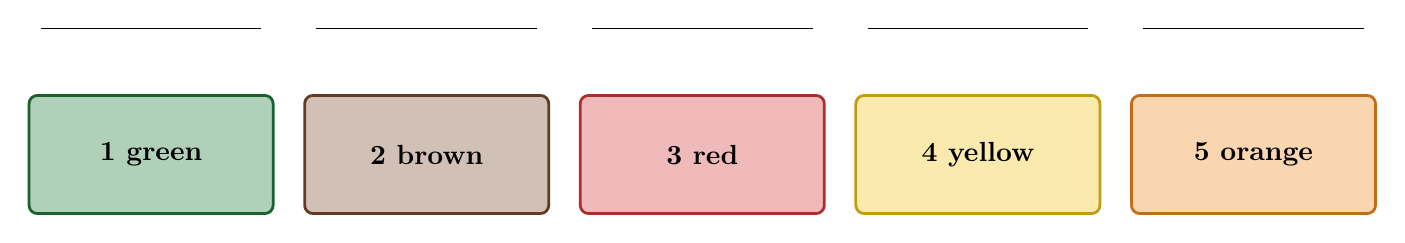
\begin{tikzpicture}
  \chair{0}{cgreen}{1 green}\chair{3.5}{cbrown}{2 brown}\chair{7}{cred}{3 red}
  \chair{10.5}{cyellow}{4 yellow}\chair{14}{corange}{5 orange}\end{tikzpicture}\end{center}}
\newcommand{\mainpuzzle}{%
  \heading{Who sat where?}
  Five animals, Bear, Fox, Owl, Rabbit and Turtle, went to a show and sat in the five coloured chairs.
  Write each animal's name above its chair.
  \fivechairs
  \begin{enumerate}\setlength{\itemsep}{2pt}
  \item Fox sat in the red chair.
  \item Owl sat on an end chair.
  \item Rabbit sat right next to Owl.
  \item Bear sat somewhere to the left of Fox.
  \item Turtle sat right next to Fox.
  \end{enumerate}
  \textbf{Done?} Cross out clue 5. How many answers are there now? Write a new clue that makes it exactly one again.}
\begin{document}
\begin{half}\mainpuzzle\end{half}
\cutline
\begin{half}\mainpuzzle\end{half}
\newpage
\begin{half}
\heading{Who sat where? (three chairs)}
Three animals, Bear, Fox and Owl, went to a show and sat in three coloured chairs.
Write each animal's name above its chair.
\begin{center}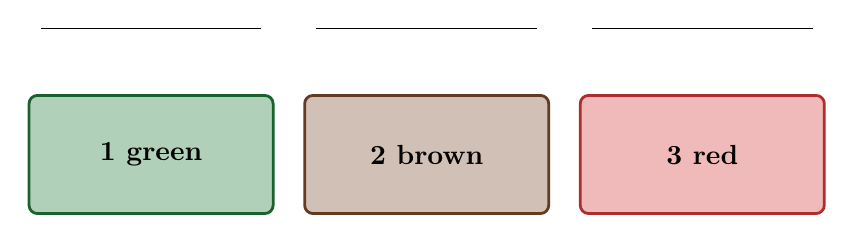
\begin{tikzpicture}
  \chair{0}{cgreen}{1 green}\chair{3.5}{cbrown}{2 brown}\chair{7}{cred}{3 red}\end{tikzpicture}\end{center}
\begin{enumerate}\setlength{\itemsep}{2pt}
\item Owl sat in the green chair.
\item Fox did not sit next to Owl.
\end{enumerate}
\textbf{Done?} Try the five-chair puzzle.
\end{half}
\cutline
\begin{half}
\heading{Who sat where? (no chair given)}
Five animals, Bear, Fox, Owl, Rabbit and Turtle, went to a show and sat in the five coloured chairs.
Write each animal's name above its chair. No clue tells you a chair straight away.
\fivechairs
\begin{enumerate}\setlength{\itemsep}{2pt}
\item Owl sat on an end chair.
\item Rabbit sat right next to Owl.
\item Fox had exactly one animal between it and Owl.
\item Bear sat somewhere to the left of Rabbit.
\item Turtle did not sit on an end chair.
\end{enumerate}
\textbf{Done?} Write your own five-chair puzzle with exactly one answer, and give it to a friend.
\end{half}
\end{document}
